\documentclass{article}

\usepackage{amsmath,amsfonts,amssymb,amsthm}
\usepackage{enumitem}
\usepackage{a4wide}
\usepackage[document]{ragged2e}
\usepackage{tikz}
\usepackage[utf8]{inputenc}
\usepackage[T1]{fontenc}
\usepackage[german]{babel}
\usepackage{hyphenat}
\usepackage{listings}
\usepackage{caption}
\usepackage{makeidx}
\usepackage{wasysym}
\usepackage{color}
\usepackage{graphicx}
\usepackage{accents}
\usepackage{stmaryrd}

\usetikzlibrary{positioning, calc}
\usetikzlibrary{decorations.pathreplacing,angles,quotes}
\usetikzlibrary{decorations.pathmorphing,snakes}
\usetikzlibrary{shapes.misc}
\usetikzlibrary{intersections,through,backgrounds}


\theoremstyle{plain}
\newtheorem{theorem}{Theorem}
\newtheorem{lemma}[theorem]{Lemma}
\newtheorem*{lemma*}{Lemma}
\newtheorem{cor}[theorem]{Korollar}
\newtheorem*{cor*}{Korollar}
\newtheorem{prop}[theorem]{Proposition}
\setlength{\parskip}{1em}

\theoremstyle{definition}
\newtheorem{definition}[theorem]{Definition}
\newtheorem*{definition*}{Definition}
\newtheorem{notation}[theorem]{Notation}
\newtheorem{bemerkung}[theorem]{Bemerkung}
\newtheorem*{bemerkung*}{Bemerkung}
\newtheorem{bsp}[theorem]{Beispiel}
\newtheorem*{remark*}{remark}
\newtheorem{remark}{remark}

\numberwithin{equation}{section}

\newcommand{\norm}[1] {
\left|\left| #1 \right|\right|
}

\newcommand{\hnorm}[1] {
\left|\left|\left| #1 \right|\right|\right|
}

\newcommand{\colvec}[1]{
\begin{pmatrix}#1\end{pmatrix}
}

\newcommand{\vect}[1]{
\begin{pmatrix}#1\end{pmatrix}
}

\newcommand{\skprod}[2]{
\left \langle #1,#2 \right \rangle
}
\newcommand{\abs}[1] {
\left| #1 \right|
}

\newcommand{\br}[1] {
\left( #1 \right)
}

\newcommand{\R}[0] {
\mathbb R
}

\newcommand{\Z}[0] {
    \mathbb Z
}

\newcommand{\N}[0] {
    \mathbb N
}

\newcommand{\srmatrix}[1] {
\left( \begin{smallmatrix} #1 \end{smallmatrix} \right)
}

\newcommand{\mtitle}[1] {
    \begin{center}
        \large{\textbf{#1}}
    \end{center}
}

\newcommand{\Index}[1]{#1\index{#1}}

\newcommand{\mim}[1] {
\underline{\textbf{#1\index{#1}}}
}

\newcommand{\C}[0]{
    \cdot
}

\newcommand{\pa}[1] {
    \par{\textbf{#1}}
}

\newcommand{\tvmark}[3] {
    \draw[] (#1,0.1+#2) -- (#1,-0.1+#2) node[anchor =north] {\small #3};
}
\newcommand{\thmark}[3] {
    \draw[] (#1+0.1,#2) -- (#1-0.1,#2) node[left] {\small #3};
}

\newcommand{\tvnmark}[3] {
    \draw[] (#1,#2-0.1) node[below] {\small #3};
}

\newcommand{\tlbar}[5]{
    \draw[thick] (#1,#2-0.1) node[below] {\small #4} -- (#1,#3) node[above] {#5};
    \draw[thick] (#1-0.1,#3) -- (#1+0.1,#3);
}



\definecolor{dkgreen}{rgb}{0,0.6,0}
\definecolor{gray}{rgb}{0.5,0.5,0.5}
\definecolor{mauve}{rgb}{0.58,0,0.82}

\lstset{frame=tb,
language=Matlab,
aboveskip=10mm,
belowskip=10mm,
showstringspaces=false,
columns=flexible,
basicstyle={\small\ttfamily},
numbers=left,
identifierstyle=\color{black},
numberstyle=\small\color{gray},
keywordstyle=\color{blue},
commentstyle=\color{dkgreen},
stringstyle=\color{mauve},
breaklines=true,
breakatwhitespace=true,
tabsize=3}

%Font
\usepackage{cmbright}
\makeindex

\begin{document}
\title{Mathematische Bildverarbeitung}
%\author{Jonas Sattler}
\date{}
\maketitle

\tableofcontents

\newpage

\section{Überblick}
    \subsection{Techniken der Bildverarbeitung}
        \begin{enumerate}[label=\textbullet]
            \item Kontrastverbesserung
            \item Entrauschen
            \item Kantendetektion
            \item Schärfen
            \item Inpainting
            \item Segmentierung (Einzlene Objekte detektieren)
            \item Registrierung (Bilder des selben Objektes in Einklang bringen)
        \end{enumerate}

    \subsection{Unser Fokus}
        \begin{enumerate}[label=\textbullet]
            \item Mathematische Beschreibung
        \end{enumerate}

    \subsection{Verwandte Vorlesungen}
        \begin{enumerate}[label=\textbullet]
            \item 3D computervision
            \item Digitale Bildanalyse
            \item Mustererkennung und Datenkompression
            \item Medical imaging
        \end{enumerate}

    \subsection{Literatur}
        \begin{enumerate}[label=\textbullet]
            \item Bredies, Lorenz : Mathematische Bildverarbeitung
            \item Aubert, Kornprobst : Mathematical Problems in Image Processing
            \item Modersitzki : Numerical Methods for Image Registration
            \item Alt : Lineare Funktionalanalysis
        \end{enumerate}

\section{Was ist ein Bild?}
    \subsection{Definition}
        \begin{minipage}[t]{0.45\linewidth}
            \mtitle{\underline{Digitale/diskrete Sicht}}
            \begin{center}
                \begin{tikzpicture}
                    \fill[black!30!white] (1,2) rectangle (1.5,2.5);
                    \draw[step=0.5,thin,draw=black] (0,0) grid (4,4);
                    \draw[thick] (0,0) rectangle (4,4);
                \end{tikzpicture}
                \captionof{figure}{Diskretes Bild}
                Darstellung als Matrix.
            \end{center}
        \end{minipage}
        \hfill\vrule\hfill
        \begin{minipage}[t]{0.45\linewidth}
            \mtitle{\underline{Kontinuierlich/analoge Sicht}}
            \begin{center}
                \begin{tikzpicture}
                    \draw[thick,->] (0,0) -- (3,0) node[anchor=west] {X};
                    \draw[thick,->] (0,0) -- (0,3) node[anchor=south] {Y};
                    \draw[thick] (0.2,0.2) rectangle (2.8,2.8);
                    \draw (1.5,2) node[] {\tiny{\textbullet}} node[anchor=west] {\small$(x,y)$};
                    \draw[] (1.5,0.1) -- node[anchor=north] {\small x} (1.5,-0.1);
                    \draw[] (0.1,2) -- node[anchor=east] {\small y} (-0.1,2);
                    \draw[|-|] (0.2,-0.4) node[anchor=north] {\small a} -- (2.8,-0.4) node[anchor=north] {\small b};
                    \draw[|-|] (-0.4,0.2) node[anchor=east] {\small c} -- (-0.4,2.8) node[anchor=east] {\small d};
                \end{tikzpicture}
                \captionof{figure}{Kontinuierliches Bild}
                Darstelllung als Funktion in zwei Veränderlichen
            \end{center}
        \end{minipage}

        \ \\

        \begin{minipage}[t]{0.47\linewidth}
            \pa{Werkzeuge:} Lineare Algebra
            \pa{Vorteile:} Endlicher Speicher
            \pa{Nachteile:} Probleme bei zoomen und drehen
        \end{minipage}
        \hfill\vrule\hfill
        \begin{minipage}[t]{0.47\linewidth}
            \pa{Werkzeuge:} Analysis
            \pa{Vorteile:} Mehr Freiheit (z.b. Kante=Linie entlang einer Unstetigkeit)
            \pa{Nachteile:} Unendlicher Speicher
        \end{minipage}

        \begin{definition*}
            Ein \mim{Bild} ist eine Funktion $u: \Omega \to F$, wobei $\Omega \subset \mathbb Z^d$ (im diskreten Fall) oder $\Omega \subset \mathbb R^d$ (im kontinuierlichen Fall).
            \begin{enumerate}
                \item[$d=2$:] Typisches 2D Bild
                \item[$d=3$:] 3D-Bild bzw. "Körper" \ \underline{oder} Video: 2D Ort + Zeit
            \end{enumerate}
            F ist der \mim{Farbraum}, Beispiele:
            \begin{enumerate}[label=\textbullet]
                \item F$=[0,1]$ oder F=$\{0,1,..., 255\}$, Graustufen
                \item F$=\{0,1\}$ schwarz/weiß
                \item F$=[0,1]^3$ oder F$=\{0,1,...,255\}^3$ Farbbilder
            \end{enumerate}
        \end{definition*}
    \subsection{Umwandlung}

        \pa{Kontinuierlich $\to$ Diskret:}\\
            \begin{minipage}[t]{0.49\linewidth}
                \
                \begin{center}
                    \begin{tikzpicture}
                        \draw (-0.5,2) node {$\Omega=$};
                        \draw[step=0.5,thin,draw=black,dotted] (0.01,0.01) grid (3.99,3.99);
                        \draw[thick] (0,0) rectangle (4,4);
                        \draw[thick] (2,2) rectangle (2.5,2.5);
                        \draw[] (2.1,2.1) -- (3,-0.3) node[anchor = south west, yshift = -7] {\small Box $B_i$};
                    \end{tikzpicture}
                \end{center}
            \end{minipage}
            \hfill\vrule\hfill
            \begin{minipage}[t]{0.49\linewidth}
                \
                \begin{center}
                    \begin{enumerate}[label=\textbullet]
                        \item $\Omega$ in Gitter zerlegen
                        \item Jede Box durch nur einen Farbwert approximieren
                        \item Etwa durch den Funktionswert im Mittelpunkt der Box
                        \item oder durch den Mittlewert in der Box:\\ $\displaystyle \frac{1}{\abs{B_i}} \C \int_{B_i}u(x)dx$
                    \end{enumerate}
                \end{center}
            \end{minipage}

                \ \\
            \pa{Diskret $\to$ Kontinuierlich:}\\
                \begin{minipage}[t]{0.49\linewidth}
                    \
                    \begin{center}
                        \begin{tikzpicture}
                            \draw (-1,2) node {$\Omega=$};
                            \draw[->] (-0.25,-0.25) -- (-0.25,4.5);
                            \draw[->] (-0.25,-0.25) -- (4.5,-0.25);
                            \draw (-0.35,4) -- (-0.15,4);
                            \draw (-0.35,0) -- (-0.15,0);
                            \draw (0,-0.35) -- (0,-0.15);
                            \draw (4,-0.35) -- (4,-0.15);                            
                            \draw[step=0.5,thin,draw=black] (0,0) grid (4,4);
                            \foreach \x in {0.25,0.75,..., 3.75}{
                                \foreach \y in {0.25,0.75,..., 3.75}{
                                    \draw (\x,\y) node {\tiny \textbullet};
                            }
                            }
                            \draw[thick] (0,0) rectangle (4,4);
                            \draw[thick] (2,2) rectangle (2.5,2.5);
                            \draw[] (2.1,2.1) -- (3,-0.7) node[anchor = south west, yshift = -7] {\small Box $B_i$};
                        \end{tikzpicture}
                    \end{center}
                \end{minipage}
                \hfill\vrule\hfill
                \begin{minipage}[t]{0.49\linewidth}
                    \
                    \begin{center}
                        \begin{enumerate}
                            \item[1.] Idee: Jeder Punkt der Box $B_i$ erhält den Funktionswert von $B_i$ aus als diskretem Pixel $\Rightarrow$ \mim{Nearest neighbour interpolation}.
                            \item[2.] Idee: Mittelpunkt von Box $B_i$ erhält den Wert von Pixel $B_i$ sonst wird interpoliert.\\
                            Grauwert $g:=$ Gewichtetes Mittel aus Grauwerten $a,b,c,d$.\\
                        \end{enumerate}

                            \begin{center}
                                \begin{tikzpicture}[scale=1.5]
                                    \draw[step = 1] (0.75,0.75) grid (3.25,3.25);
                                    \foreach \x in {1.5,2.5}{
                                        \foreach \y in {1.5,2.5}{
                                            \draw (\x,\y) node {\tiny \textbullet};
                                    }
                                    }
                                    \draw (1.5,2.5) node[anchor=north west] {a};
                                    \draw (2.5,2.5) node[anchor=south west] {b};
                                    \draw (1.5,1.5) node[anchor=north west] {c};
                                    \draw (2.5,1.5) node[anchor=north west] {d};

                                    \draw (1.5,1.5) rectangle (2.5,2.5);
                                    \draw (1.45,2.15) -- (1.55,2.15);
                                    \draw (1.8,2.45) -- (1.8,2.55);
                                    \draw[decorate,decoration={brace,amplitude=2pt}] (1.5,2.6) -- node[anchor=south] {\small $\alpha$} (1.8,2.6);
                                    \draw[decorate,decoration={brace,amplitude=2pt}] (1.4,2.15) --node[anchor=east] {\small $\beta$} (1.4,2.5);
                                    \draw (1.8,2.15) node {\tiny \textbullet} node[anchor=west, xshift=-2] {\small p};
                                    \draw[decorate,decoration={brace,amplitude=4pt}] (1.5,2.9) -- node[anchor= south west,yshift = 2] {\small 1} (2.5,2.9);
                                    \draw[decorate,decoration={brace,amplitude=4pt}] (1.1,1.5) -- node[anchor= south east, xshift=-2] {\small 1} (1.1,2.5);
                                \end{tikzpicture}
                            \end{center}

                            \small{$g=(1-\alpha) \C (1-\beta) \C a + \alpha \C (1- \beta) \C b + (1-\alpha) \C \beta \C c + \alpha \C \beta \C d$}\\
                            Dieses wird \mim{Bilinear interpolation} genannt.
                    \end{center}
                \end{minipage}

    \subsection{Beispiel Rotation}
        \begin{center}
            \begin{tikzpicture}%TODO redo
                \draw (0,0.1) -- node[anchor=center] {\tiny \textbullet} node[anchor=north] {\tiny $0$} (3,0.1);
                \draw  (4,0.1) node  {$\overset{\text{\footnotesize um $\alpha$ drehen}}{\Rightarrow}$};
                \draw (6.5,0.1) -- ++(30:1.5);
                \draw (6.5,0.1) node[anchor=center] {\tiny \textbullet} node[anchor=north] {\tiny $0$} -- ++(210:1.5);
                \draw[dotted] (5,0.1) -- (8,0.1);
                \draw (7,0.1) arc[radius=0.5,start angle=0,end angle=30]  node[anchor = north west] {\tiny $\alpha$};
            \end{tikzpicture}
        \end{center}

        \pa{1. Fall, kontinuierliches Bild}\\
            Sei $u$ das alte Bild und $v$ das neue Bild, dann ist die Drehung gegeben durch eine \mim{Drehmatrix}:

            \[D_\varphi \in \R^{d \times d}, D_\varphi=\srmatrix{cos(\varphi) \ -sin(\varphi) \\ sin(\varphi) \ cos(\varphi)}\]

            Damit folgt, dass $D(u)= D_\varphi \Omega$ und $v(x)=u(\underbrace{D_\varphi^{-1}x}_{\in \Omega}) = u(D_{-\varphi}x)$. ($D(u)$ ist die \mim{Domain} von $u$)

        \pa{2. Fall, diskretes Bild}\\
            Dieses ist problematisch, denn I.A. $x \in \Z^d$, aber $D_\varphi x \not \in \Z^d$.

            \begin{center}
                \begin{tikzpicture}
                    \foreach \x in {0,1,2,3}{
                            \draw (0.5*\x,0) node {\tiny \textbullet};
                    }
                    \draw[decorate,decoration={brace,amplitude=4pt,mirror}] (-0.1,-0.1) -- node[anchor= north] {\small $\subset \Z^d$} (1.6,-0.1);
                    \draw[->] (1.75,0) -- (2,0);
                    \draw[step=0.5, shift={(2.25,0.25)}] (0,0) grid (2,-0.5);
                    \foreach \x in {0,1,2,3}{
                        \draw[shift={(2.5,0)}] (0.5*\x,0) node {\tiny \textbullet};
                    }
                    \draw[decorate,decoration={brace,amplitude=4pt,mirror}] (2.15,-0.4) -- node[anchor= north] {\small $\subset \R^d$} (4.35,-0.4);
                    \draw[->] (4.5,0) -- node[above] {\small $D_\varphi$} (4.75,0);
                    \draw[step=0.5, shift={(5,0.25)},rotate around = {45:(1,-0.25)}] (0,0) grid (2,-0.5);
                    \foreach \x in {0,1,2,3}{
                        \draw[shift={(5.25,0)},rotate around = {45:(0.75,0)}] (0.5*\x,0) node {\tiny \textbullet};
                    }
                    \draw[decorate,decoration={brace,amplitude=4pt,mirror}] (4.9,-1) -- node[anchor= north] {\small $\subset \R^d$} (7.1,-1);
                    \draw[->] (7.25,0) -- node[above] {\small rastern} (7.5,0);
                    \draw[->] (4.5,0) -- node[above] {\small $D_\varphi$} (4.75,0);
                    \draw[step=0.5, shift={(8,0.25)},rotate around = {45:(1,-0.25)}] (0,0) grid (2,-0.5);
                    \foreach \x in {0,1,2,3}{
                        \draw[shift={(8.25,0)},rotate around = {45:(0.75,0)}] (0.5*\x,0) node {\tiny \textbullet};
                    }
                    \draw[dotted,step=0.5] (7.9,1) grid (10.1,-1);
                    \draw[decorate,decoration={brace,amplitude=4pt,mirror}] (7.9,-1.2) -- node[anchor= north] {\small $\subset \Z^d$} (10.1,-1.2);
                \end{tikzpicture}
            \end{center}

            Weiterhin ist $v(x)=u(D_\varphi^{-1} x)$, wobei der konkrete Wert durch Interpolation bestimmt wird.

            \begin{center}
                \begin{tikzpicture}
                    %TODO Images
                    \draw[line width = 0.5cm] (0,0) -- (4,0);
                    \draw[->] (4.3,-0.4) -- node[sloped,below] {Bilinear} (7,-2);
                    \draw[->] (4.3,0.4) -- node[sloped,above] {Nearest neighbour} (7,2);                    
                \end{tikzpicture}
            \end{center}


\section{Histogramme und deren Anwendungen}

    \subsection{Histogramme}
        Sei $u:\Omega \to F$ ein diskretes Bild, dann heißt die Abbildung
        \[H_u : F \to \N_0\]
        \[F \ni k \mapsto \# \{x \in \Omega | u(x) = k\}\]
        \mim{Histogramm} des Bildes $u$. Dieses gibt an, wie often die Farbe $k$ im Bild vorhanden ist.\\
        Damit gilt auch:
        \[\sum_{k \in F}H_u(k)=\abs{\Omega} \text{, also die Anzahl der Pixel}\]
        \begin{bemerkung*}
            Manchmal betrachtet man die relative Häufigkeit $\displaystyle \tilde H_u(k) = \frac{H_u(k)}{\abs{\Omega}}$.
        \end{bemerkung*}

        \pa{\large Beispiel:}

        \begin{center}
            \begin{tikzpicture}
                \draw (0,0) node {$\Omega=$};
                \draw[fill = black] (1.05,0.95) rectangle (1.95,0.05);
                \draw[fill = black] (2.05,0.95) rectangle (2.95,0.05);
                \draw[fill = black!30] (1.05,-0.05) rectangle (1.95,-0.95);
                \draw[fill = white] (2.05,-0.05) rectangle (2.95,-0.95);
                \draw (1,1) grid (3,-1);
                \draw[->] (3.25,0) -- (3.5,0);
                \draw[->] (4,-1.25) -- (8,-1.25) node[right] {$F$};
                \draw[->] (4,-1.25) -- (4,1.5);
                \tvmark{5}{-1.25}{black}
                \tvmark{6}{-1.25}{grey}
                \tvmark{7}{-1.25}{white}
                \thmark{4}{-0.25}{1}
                \thmark{4}{0.75}{2}
                \draw (5,0.75) node {\textbullet};
                \draw (6,-0.25) node {\textbullet};
                \draw (7,-0.25) node {\textbullet};                
            \end{tikzpicture}
        \end{center}

        Für kontinuierliche Bilder wird  das allgemeinere Konzept von einem \mim{Maß} benötigt:
        \begin{center}
            \begin{tikzpicture}
                \draw (0,0) node[left] {$A \subset F, \ \mathcal H_u := \abs{u^{-1}(A)}$};
                \draw[->,text width = 4.5cm] (0,0.1) -- (0.75,0.75) node[right] {\small \underline{Diskretes Bild:}\\ Anzahl der Elemente in $u^{-1}(A)$};
                \draw[->,text width = 4.5cm] (0,-0.1) -- (0.75,-0.75) node[right] {\small \underline{Kontinuierliches Bild:}\\ Volumen von  $u^{-1}(A)$};
            \end{tikzpicture}
        \end{center}

        Zusammenhang zum vorherigen: $\displaystyle \mathcal H_u(A) = \sum_{k \in A} H_u(k)$.
        Man sagt dann, dass $U_u$ eine \mim{Dichte} zum Maß $\mathcal H_u$ sei. Diese kann auch in kontinueirlichen existieren:

        \begin{center}
            \begin{tikzpicture}
               \draw[->] (0,0) -- (8,0) node[right] {$F$};
               \draw[->] (0,0) -- (0,4);
               \draw[thick] plot [smooth, tension = 0.8] coordinates {(0,1) (2,2) (4,0.75) (5.5,2.5) (7,0)};
            \end{tikzpicture}
        \end{center}

    \subsection{Anwendung: Kontrastverbesserung}
        \pa{Problem \& Idee:} Falls das Bild nur einen kleinen Teil von $F$ nutzt, kann der Kontrast verbessert werden, indem man das Bild auf ganz $F$ verteilt.
        \begin{center}
            \begin{tikzpicture}
               \draw[->] (0,0) node[yshift=-4, xshift = -4] {0} -- (4.2,0) node[right] {$F$};
               \draw[->] (0,0) -- (0,2);
               \draw[thick] plot [smooth, tension = 0.8] coordinates {(1.5,0) (1.75,0.75) (2,0.5) (2.25,1.25) (2.5,0)};
               \tvmark{1.5}{0}{$k_{min}$}
               \tvmark{2.5}{0}{$k_{max}$}
               \draw[->,thick] (4.25,1) -- (4.75,1);
               \draw[->] (5,0) node[yshift=-4, xshift = -4] {0} -- (9.2,0) node[right] {$F$};
               \draw[->] (5,0) -- (5,2);
               \draw[thick,shift={(5,0)}] plot [smooth, tension = 0.8] coordinates {(0,0) (1,0.75) (2,0.5) (3,1.25) (4,0)};
               \tvmark{9}{0}{$N$}
            \end{tikzpicture}
        \end{center}

        \begin{center}
            \begin{tikzpicture}
                \draw[->] (0,0) node[below] {$\Omega$} to[bend left] node[above] {\small originales Bild} (1.8,0);
                \draw (2,0) node[below] {$F$};
                \draw[->] (2.2,0) to[bend left] node[above] {\small Zauberei $T$} (4,0) node[below] {$F$};
                \draw[->] (0,-0.5) to[bend right] node[below] {\small Bild mit besserem Kontrast} (4,-0.5);
                \draw[text width = 2.3cm] (5,0) node[right] {\small $v = T \circ u$\\ $v(k)=T(u(k)) $};
            \end{tikzpicture}
        \end{center}

        \pa{1. Idee, Kontrastdehnung:}\\
        $T$ ''lineare'' Abbildung, so dass $T(k_{min})=0$ und $T(k_{max})=N$:
        \[T(k) = \frac{k - k_{min}}{k_max} N \text{, Kontinuierlicher Farbraum}\]
        \[T(k) = \left[\frac{k - k_{min}}{k_max} N \right] \text{, Diskreter Farbraum}\]

        \underline{Beispiel:}

        \begin{center}
            \begin{tikzpicture}
                \draw[->] (0,0) node[yshift=-4, xshift = -4] {0} -- (6,0) node[right] {$F$};
                \draw[->] (0,0) -- (0,3);
                \tlbar{0.75}{0}{1}{20}{4}
                \tlbar{1.5}{0}{1.25}{40}{6}
                \tvnmark{2.25}{0}{...}
                \tlbar{3}{0}{1.75}{99}{10}
                \tlbar{3.4}{-0.3}{2.75}{100}{20}
                \tlbar{3.8}{0}{2.25}{101}{15}
                \tlbar{4.2}{-0.3}{1.125}{102}{5}
                \tvnmark{4.8}{0}{...}
                \tvmark{5.5}{0}{255}
                \draw[->, thick, text width = 2cm] (6.5,1.5) -- node[above] {\footnotesize Lineare Transformation $T$} (7.5,1.5);
                \draw[->] (8,0) node[yshift=-4, xshift = -4] {0} -- (13,0) node[right] {$F$};
                \draw[->] (8,0) -- (8,3);
                \tlbar{8.25}{0}{1}{3}{4}
                \tvnmark{8.75}{0}{...}
                \tlbar{9.25}{0}{1.75}{64}{6}
                \tvnmark{9.75}{0}{...}
                \tlbar{10.25}{0}{1.75}{243}{10}
                \tlbar{10.75}{-0.3}{2.75}{246}{20}
                \tlbar{11.25}{0}{2.25}{249}{15}
                \tlbar{11.75}{-0.3}{1.125}{252}{5}
                \tvmark{12.4}{0}{255}
                \draw[] (1.5,2.25) node[] {$\abs{\Omega}=60$};
                \draw (10.5,-0.8) node[below] {\footnotesize $k_{min} =19, \ k_{max}=103$};
            \end{tikzpicture}
        \end{center}

        \pa{2. Idee nicht-lineare Kontrastdehnung}\\
            Diesesmal setzen wir $\displaystyle T(k) =\left[ \frac{N}{\abs{\Omega}} \sum_{l=0}^{k}H_u(l) \right]$ für einen diskreten Farbraum und erhalten:

            \begin{center}
                \begin{tikzpicture}
                    \draw[->] (0,0) node[yshift=-4, xshift = -4] {0} -- (8,0) node[right] {$F$};
                    \draw[->] (0,0) -- (0,3);
                    \draw[decorate,decoration={brace,amplitude=2pt,mirror}] (0,-0.2) -- node[below] {\small $\frac{4}{60} N$} (1,-0.2);
                    \tlbar{1}{0}{1}{}{4}
                    \draw[decorate,decoration={brace,amplitude=2pt,mirror}] (1,-0.2) -- node[below] {\small $\frac{6}{60} N$} (2.5,-0.2);
                    \tlbar{2.5}{0}{1.25}{}{6}
                    \draw[decorate,decoration={brace,amplitude=2pt,mirror}] (2.5,-0.2) -- node[below] {\small $\frac{10}{60} N$} (4.5,-0.2);
                    \tlbar{4.5}{0}{1.75}{}{10}
                    \draw[decorate,decoration={brace,amplitude=2pt,mirror}] (4.5,-0.2) -- node[below] {\small $\frac{20}{60} N$} (7,-0.2);
                    \tlbar{7}{0}{2.5}{}{20}
                    \tvnmark{7.5}{0}{...}
                \end{tikzpicture}
            \end{center}
        $T$ lässt sich auch alternativ ausdrücken durch:
        \[ T(k)=\left[ \mathcal H_u(\{0,...,k\}) \right] \]
        Und somit folg dass für den kontinueirlichen Fall $T$ durch
        \[ T(k) = \frac{N}{\abs{\Omega}} \mathcal H_u((0,k))\]
        definiert werden kann. Allgemein heißt der Prozess \mim{Histogramm - equalisation}.
    \subsection{Anwendung: SW-Konvertierung}
        Aufgabe: Graustufenbild $\to$ SW-Bild.\\
        Nüzlich etwa bei Objekterkennung/Segmentierung.

        Idee: Das Histogramm an einem gewissen \mim{Schwellenwert} $t$ spalten:

        \begin{center}
            \begin{tikzpicture}
                \fill[black!80](0.1,0) rectangle (3.5,3);
                \fill [white] (0.05,0) -- plot [smooth, tension = 0.7] coordinates {(1,0) (2,1.7) (3,1) (4.5,2) (7,0)} -- (7.5,3.5) -- (0.1,3.5)  -- cycle;
                \draw[->] (0,0) node[below] {dunkel} -- (8,0) node[below] {hell} node[right] {$F$};
                \draw[->] (0,0) -- (0,4);
                \draw[thick] plot [smooth, tension = 0.7] coordinates {(1,0) (2,1.7) (3,1) (4.5,2) (7,0)};
                \draw[densely dotted,thick] (3.5,-0.2) node[below] {$t$} -- (3.5,3);
            \end{tikzpicture}
        \end{center}
        Also setze nun für $t \in F$:
        \[\text{schwarz} = \left\{k \in F | k \leq t \right\} \]
        \[\text{weiß} = \left\{k \in F | k >t \right\}\]
        Graustufenbild $u$ $\longrightarrow$ schwarz/weiß Bild $\tilde u$:

        \[\tilde u(x) = \begin{cases}
            0, \ u(x) \in \text{schwarz}\\
            1, \ u(x) \in \text{weiß}
        \end{cases} \Rightarrow \ \tilde F = \{0,1\}\]

        \pa{Methoden um diesen Schwellenwert zu wählen:}

        \begin{enumerate}
            \item \mim{Shape based Methods}:\\
            Falls das Histogramm von $u$ \mim{bimodal} ist, also die Form:
            \begin{center}
                \begin{tikzpicture}
                    \draw[->] (0,0) -- (4,0) node[right] {$F$};
                    \draw[->] (0,0) -- (0,2);
                    \draw[thick] plot [smooth, tension = 0.6] coordinates {(0.5,0) (1.3,1) (2,0.3) (2.5,1.5) (3,0)};
                    \draw (1.3,-0.1) node[below] {\small $k_{max 1}$} -- (1.3,1);
                    \draw (2,-0.35) node[below] {\small $k_{min}$} -- (2,0.3);
                    \draw (2.5,-0.1) node[below] {\small $k_{max 2}$} -- (2.5,1.5);
                \end{tikzpicture}
            \end{center}
            hat, dann wähle:
            \[t:=k_{min}\]
            \[\text{oder} \ t:= \frac{k_{max 1} + k_{max 2}}{2}\]
            \item \mim{Otsu's Verfahren} (1979):\\
            Vorher einige Definitionen.\\
            Die \mim{Masse}:
            \[m_{\text{schwarz}} := \sum_{k \in \text{schwarz}} H_u(k)\]
            \[m_{\text{weiß}} := \sum_{k \in \text{weiß}} H_u(k)\]
            Der \mim{Mittlewert}:
            \[\mu_{\text{schwarz}} := \frac{\displaystyle \sum_{k_ \in \text{schwarz}} k \C H_u(k) }{\displaystyle \sum_{k_ \in \text{schwarz}}H_u(k)} = \frac{\displaystyle \sum_{k_ \in \text{schwarz}} k \C H_u(k) }{m_{\text{schwarz}}}\]
            \[\mu_{\text{weiß}} := \frac{\displaystyle \sum_{k_ \in \text{weiß}} k \C H_u(k) }{\displaystyle \sum_{k_ \in \text{weiß}}H_u(k)} = \frac{\displaystyle \sum_{k_ \in \text{weiß}} k \C H_u(k) }{m_{\text{weiß}}}\]
            Die \mim{Varianz}:
            \[\sigma^2_{\text{schwarz}} = \sum_{k \in \text{schwarz}} (k - \mu_{\text{schwarz}})^2 \C H_u(k)\]
            \[\sigma^2_{\text{weiß}} = \sum_{k \in \text{weiß}} (k - \mu_{\text{weiß}})^2 \C H_u(k)\]
            Nun lautet Otsu's Methode: $\sigma^2_{\text{schwarz}} + \sigma^2_{\text{weiß}} \overset{t}{\rightarrow} \text{min}$.
            \item \mim{Median}:\\
            Wähle $t$ so dass $m_{\text{schwarz}} = m_{\text{weiß}}$.
            \item \mim{Isodata Algorithmus} (1970s):\\
            Wähle t so, dass $\displaystyle t = \frac{\mu_{\text{schwarz}} - \mu_{\text{weiß}}}{2} =: f(t)$.\\
            Diese Gleichung ist bereits eine \mim{Fixpunktgleichung} und eine Lösung kann, etwa mit einer \mim{Fixpunktiteration} approximiert werden, das heißt $t_{n+1} := f(t_n)$.
            \begin{center}
                \begin{tikzpicture}%TODO fixpunkt iteration in Grafik?
                    \draw[->] (0,0) node[below] {0} -- (0,5) node[above] {y};
                    \draw[->] (0,0) -- (5,0)node[right] {x};
                    \draw (-0.1,4.5) node[left] {N} -- (4.5,4.5);
                    \draw (4.5,-0.1) node[below] {N} -- (4.5,4.5);
                    \draw[name path = P1] (-0.1,-0.1) -- node[below,sloped, pos = 0.7] {$y=x$} (4.6,4.6);
                    \coordinate (A) at (0.5,0.5);
                    \draw[thick, name path = P2] plot [smooth, tension = 0.8] coordinates {(0,0.5) (0.5,0.7) (1,1.1) (2, 1.7) (2.8, 3.1) (4.5,4.25)};
                    \draw (3,3.7) node[rotate = 35] {$y = f(x)$};
                    \fill[name intersections={of=P1 and P2}]
                    (intersection-1) circle (1.5pt) node {}
                    (intersection-2) circle (1.5pt) node {}
                    (intersection-3) circle (1.5pt) node {};
                \end{tikzpicture}
            \end{center}
        \end{enumerate}

        \pa{Matlab code}:\\
        \begin{lstlisting}
u=imread('liftingbody.png');
t=greythresh(u);%uses Otsu's method
v=im2bn(u,t);
imshow(v);
        \end{lstlisting}

        Einige dieser Verfahren können auch erweitert werden, so dass ein Graustufenbild nicht nur in zwei, sondern in $M$ Farben zerlegt werden kann. Im allgemeinen werden dann $M-1$ thresholds benötigt.

        \begin{enumerate}
            \item \pa{Shape based}:\\
            \begin{center}
                \begin{tikzpicture}
                    \draw (0,0) -- (0,2);
                    \draw (0,0) -- (6,0);
                    \draw[thick, name path = P2] plot [smooth, tension = 0.7] coordinates {(0.5,0) (1,1) (1.5,0.2) (2, 0.9) (2.5, 0.5) (3.25,1.5) (4,0.5) (4.5,1.2) (5,0)};
                    \draw (1,-0.1) node[below] {$t_1$} -- (1,1);
                    \draw (2,-0.1) node[below] {$t_2$} -- (2,0.9);
                    \draw (3.25,-0.1) node[below] {$t_3$} -- (3.25,1.5);
                    \draw (4.5,-0.1) node[below] {$t_4$} -- (4.5,1.2);
                \end{tikzpicture}
            \end{center}
            \ \\
            \item \pa{Otsu's Verfahren}:\\
            Farbklassen:
            \[ F_1 = \{ k : k \leq t_1\}\]
            \[ F_2 = \{ k : t_1 < k \leq t_2\}\]
            \[\vdots\]
            \[ F_M = \{ k : t_{M-1} < k \}\]
            Und wie zuvor: $\sigma_1^2 + ... + \sigma_M^2 \to $ min
            \item \pa{Median}:\\
            Zerteile $F$ in M Quantile gleicher Masse.
            \item \pa{Isodata}:\\ 
            Hierzu existiert keine Bekannte Verallgemeinerung auf $M$ Farbklassen.
        \end{enumerate}

        \pa{Matlab code}:\\
        \begin{lstlisting}
u=imread('Circles Bright Dark.png');
t=multithresh(u,M-1);
v=imquantize(u,t);
w=label2rgb(u,t);
imshow(w);
        \end{lstlisting}

\section{Einfache \Index{morphographisch Operationen}}
        S/W Bild:
        \begin{center}
            \begin{tikzpicture}
                \draw (0,0) node[left] {$A=$} node[right] {
\includegraphics[scale = 0.2]{Bild1.png}};
            \end{tikzpicture}
        \end{center}
        \mim{Strukturelement}:
        \begin{center}
            \begin{tikzpicture}[scale = 2]
                    \draw[->] (0,-1) -- (0,0) node {\tiny \textbullet} -- (0,1);
                    \draw[->] (-1,0) -- (0,0) -- (1,0);
                    \fill[black!30, opacity = 0.6] (0,0) circle (0.5);
                    \draw (0,0) circle (0.5);
                    \draw (-1.1,0) node[left] {$B=$};
            \end{tikzpicture}
        \end{center}

    \subsection{Verknüpfungen von A und B}
        \[A+B := \{a + b : a \in A, b \in B\}\]
        Diese wird \mim{dilation} genannt.\\
        Anschaulich wird an jeden schwarzen Punkt des Bildes $A$ das Struktur element $B$ gelegt.
        \begin{center}
            \begin{tikzpicture}
                \draw (0,0) node[left] {$A+B=$} node[right] {
\includegraphics[scale = 0.2]{Bild1dil.png}};
            \end{tikzpicture}
        \end{center}
        Bild erzeugt in Matlab durch:\\
        \begin{lstlisting}
I=imread('Bild1.png');
se=strel('disk',40,8);
I2=imcomplement(imdilate(imcomplement(I),se));%Es wird das Komplement des Bildes gebildet, damit das Strukturelement auf den schwarzen bereich angewendet wird
imshow(I2);
        \end{lstlisting}

        \[A-B := \{a : a + B \subset A\}\]
        Diese wird \mim{erosion} genannt.\\
        Anschaulich werden die schwarzen Bereiche des Bildes gesucht, in die das Strukturelement hinein passt.
        \begin{center}
            \begin{tikzpicture}
                \draw (0,0) node[left] {$A-B=$} node[right] {
\includegraphics[scale = 0.2]{Bild1erode.png}};
            \end{tikzpicture}
        \end{center}

        Bild erzeugt in Matlab durch:\\
        \begin{lstlisting}
I=imread('Bild1.png');
se=strel('disk',20,8);
I2=imcomplement(imerode(imcomplement(I),se));
imshow(I2);
        \end{lstlisting}

        Es ist schnell zu erkennen das $A \neq (A+B)-B$, deshalb wird eine neue Operation eingeführt:
        \[A \bullet B := (A+B)-B\]
        Dieses wird \mim{schließen} gennant und wird etwa genutzt um Löcher, z.b. Rauschen, in einem Bild zu entfernen. Im Beispiel Bild ist zu sehen, dass das obere Fenster nicht mehr vorhanden ist.
        \begin{center}
            \begin{tikzpicture}
                \draw (0,0) node[left] {$A \bullet B=$} node[right] {
\includegraphics[scale = 0.2]{Bild1close.png}};
            \end{tikzpicture}
        \end{center}

        Bild erzeugt in Matlab durch:\\
        \begin{lstlisting}
I=imread('Bild1.png');
se=strel('disk',20,8);
I2=imcomplement(imdilate(imcomplement(I),se));
I3=imcomplement(imerode(imcomplement(I2),se));
imshow(I3);
        \end{lstlisting}

        Es existiert auch die Umgekehrt Operation:
        \[ A \circ B := (A-B)+B\]
        Diese wird \mim{öffnen} gennant.

        Diesmal mit einem neuen Beispiel:

        \begin{center}
            \begin{tikzpicture}
                \draw (0,0) node[left] {$A=$} node[right] {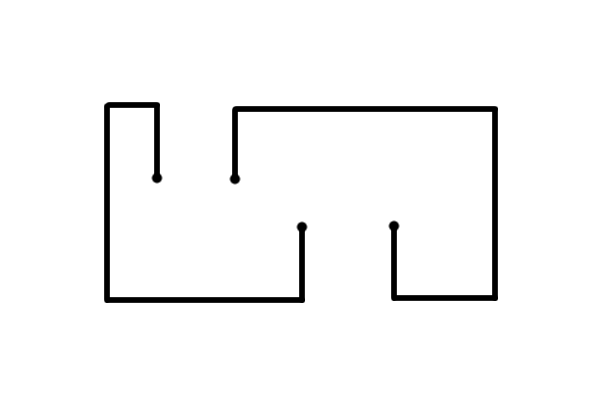
\includegraphics[scale = 0.2]{Bild2.png}};
            \end{tikzpicture}
        \end{center}

        \begin{center}
            \begin{tikzpicture}
                \draw[->] (0,-1) -- (0,0) node {\tiny \textbullet} -- (0,1);
                \draw[->] (-1,0) -- (0,0) -- (1,0);
                \fill[black!60, opacity = 0.6] (-0.05,-0.7) rectangle (0.05,0.7);
                \draw (-0.05,-0.7) rectangle (0.05,0.7);
                \draw (-1.1,0) node[left] {$B=$};
            \end{tikzpicture}
        \end{center}

        \begin{center}
            \begin{tikzpicture}
                \draw (0,0) node[left] {$A \circ B =$} node[right] {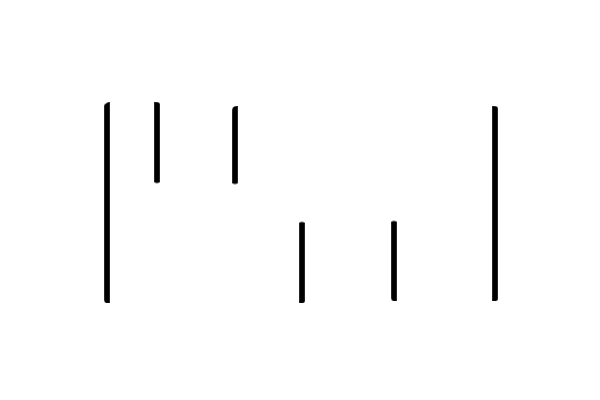
\includegraphics[scale = 0.2]{Bild2open.png}};
            \end{tikzpicture}
        \end{center}

        Bild erzeugt in Matlab durch:\\
        \begin{lstlisting}
I=imread('Bild2.png');
se=strel('line',10,90);
I2=imcomplement(imerode(imcomplement(I),se));
I3=imcomplement(imerode(imcomplement(I2),se));
imshow(I3);
        \end{lstlisting}

\section{Entrauschen: Filter \& Co.}
    \subsection{Rauschen}
        \mim{Rauschen}: Ungewollte Störungen in einem Bild
        \begin{enumerate}[label = \textbullet]
            \item punktweise
            \item zufällig
            \item unabhängig
            \item additiv (bei multiplikativem Rauschen $log$ anwenden)
        \end{enumerate}

        Notation:
        \begin{center}
            \begin{tikzpicture}
                \draw (0,0) rectangle (2,2);
                \draw (1,0) node[below] {\small Sauberes Bild};
                \draw (1,1) node[] {\LARGE $f_0$};
                \draw[->] (2.1,1) -- node[above] {\small $+$ Rauschen} (3.9,1);
                \draw (4,0) rectangle (6,2);
                \draw (5,0) node[below] {\small Gestörtes Bild};
                \draw (5,1) node[] {\LARGE $f$};
                \draw[->] (6.1,1) -- node[above] {\small Entrauschen} (7.9,1);
                \draw (8,0) rectangle (10,2);                
                \draw (9,0) node[below] {\small Resultat};
                \draw (9,1) node[] {\LARGE $u$};
            \end{tikzpicture}
        \end{center}

        Wie gut das entrauschte Bild $u$ das saubere Bild $f_0$ beschreibt wird durch Normen gemessen.
	    \begin{align*}
        &\norm{f-f_0}, \text{Rauschen}\\
        &\norm{u-f_0}, \text{\mim{Absoluter Fehler}}\\
        &\frac{\norm{u-f_o}}{\norm{f-f_0}}, \text{\mim{Relativer Fehler} im Vergleich zum Rauschen}\\
        &\frac{\norm{u-f_o}}{\norm{f_0}}, \text{Relativer Fehler im Vergleich zum Signal}
        \end{align*}
        
        Typischerweise ist die gewählte Norm:
        \[\norm{f} = \norm{f}_2 = \sqrt{\int_{\Omega} \abs{f(x)}^2 dx}\]
        oder im diskreten:
        \[\norm{f}_2=\sqrt{\sum_{x \in \Omega} \abs{f(x)}^2}\]

        Eng verwandt ist die \mim{Signal to noise ratio} (SNR):
        \[log(\underbrace{\frac{\norm{f_0}_2}{\norm{u-f_0}_2}}_{\in \ [1,\infty)}) \in [0,+\infty), \text{ wobei $0$ schlecht und $+\infty$ gut ist.}\]
    \subsection{Glättungsfilter}
        Grundidee: (zur Vereinfachung in 1D)
        \begin{center}
            \begin{tikzpicture}
                \draw (0,0) node[left] {$f_0$:};
                \draw[thick] plot [smooth, tension = 0.7] coordinates {(0,0) (1.75,1.5) (3.5,0.5) (6,2) (9,0) (11,0.5)};
                \draw[->,thick] (-0.3,-0.5) -- node[left] {Rauschen} (-0.3,-2);
                \draw (0,-2.5) node[left] {$f$:};                
                \draw[thick, name path = P2,shift = {(0,-2.5)}] plot [smooth, tension = 0.7] coordinates {(0,0) (1.75,1.5) (3.5,0.5) (6,2) (9,0) (11,0.5)};
                \draw[name path = P1, draw = none] (0,-1.1) -- (3,-1.1);
                \draw[name intersections={of = P1 and P2},red,thick]
                (intersection-1) edge[bend right] ++(0.3,0.5) ++(0.3,0.5) edge[bend right] (intersection-2);
                \draw[name path = P3,draw = none] (3,-2.3) -- (5,-1.2);
                \draw[name intersections={of = P3 and P2},red,thick]
                (intersection-1) edge[bend left] ++(0.3,-0.3) ++(0.3,-0.3) edge[bend left] (intersection-2);
                \draw[] (2,-0.9) -- ++(0.5,-0.1) node[right] {\small Störungen} (3.5,-2.1) -- ++(-0.5,0.9);
                \draw (0,-5) node[left] {$f$:};
                \draw[thick, name path = P4,shift = {(0,-5)}] plot [smooth, tension = 0.7] coordinates {(0,0) (1.75,1.5) (3.5,0.5) (6,2) (9,0) (11,0.5)};
                \draw[name path = P5, shift = {(0,-2.5)}, draw = none] (0,-1.1) -- (3,-1.1);
                \draw[name intersections={of = P4 and P5},red,thick]
                (intersection-1) edge[bend right] node[black,pos=0] {\small \textbullet} ++(0.3,0.5) ++(0.3,0.5) edge[bend right] node[black,pos=1] {\small \textbullet}  node[black,pos=0] {\small \textbullet} (intersection-2);
                \draw[name path = P6, shift = {(0,-2.5)}, draw = none] (3,-2.3) -- (5,-1.2);
                \draw[name intersections={of = P4 and P6},red,thick]
                (intersection-1) edge[bend left] node[black,pos=0] {\small \textbullet} ++(0.3,-0.3) ++(0.3,-0.3) edge[bend left] node[black,pos=1] {\small \textbullet}  node[black,pos=0] {\small \textbullet} (intersection-2);
                \draw[decorate,decoration={brace,amplitude=2pt,mirror}] (1.4,-3.7) -- (2.2,-3.7);
                \draw[thick] (1.8,-3.8) -- (1.8,-4.3) node[below] {\small \framebox{Mittelwert}};
                \draw[->,thick,double] (1.6,-5) -- (0.4,-5);
                \draw[->,thick,double] (2,-5) -- (3.2,-5);
                \draw[->,thick] (1.8,-5.1) -- (1.8,-5.7);
                \draw (0,-7.5) node[left] {$u$:};
                \draw[->,thick] (-0.3,-5.5) -- node[left] {Entrauschen} (-0.3,-7);
                \draw[thick, name path = P7,shift = {(0,-7.5)}] plot [smooth, tension = 0.7] coordinates {(0,0) (1.75,1.5) (3.5,0.5) (6,2) (9,0) (11,0.5)};
                \draw[name path = P8, shift = {(0,-5)}, draw = none] (0,-1.2) -- (3,-1.2);
                \draw[name intersections={of = P7 and P8},red,thick]
                plot [smooth,tension=0.7] coordinates {(intersection-1) ($(intersection-1) + (0.5,0.35)$) (intersection-2)};
                \draw[name path = P9, shift = {(0,-5)}, draw = none] (3,-2.25) -- (5,-1.15);
                \draw[name intersections={of = P7 and P9},red,thick]
                plot [smooth,tension=0.7] coordinates {(intersection-1) ($(intersection-1) + (0.45,0.05)$) (intersection-2)};
            \end{tikzpicture}
        \end{center}

        \begin{equation} \label{eq:5.1}
            u(k):=\alpha \cdot f(k-1) + \beta \cdot f(k) + \gamma \cdot f(k+1)
        \end{equation}
        wobei:
        \begin{equation} \label{eq:5.2}
            \alpha + \beta + \gamma = 1
        \end{equation}

        Schematisch bedeutet \eqref{eq:5.1}:
        
        \begin{center}
            \begin{tikzpicture}
                \draw (0,-0.5) node[left] {\large f:};
                \draw[thick] (0.5,0) grid (6.5,-1);
                \draw (0.5,-0.5) node {\LARGE ...};
                \draw (6.5,-0.5) node {\LARGE ...};
                \draw (1.5,0) node[above] {\dots};
                \draw (2.5,0) node[above] {k-1};
                \draw (3.5,0) node[above] {k};
                \draw (4.5,0) node[above] {k+1};
                \draw (5.5,0) node[above] {\dots};
                \draw (0.5,-2.5) node {\LARGE ...};
                \draw (6.5,-2.5) node {\LARGE ...};

                \draw[->,red] (1.6,-1.1) -- node[left] {\tiny $\alpha$} (2.4,-1.9);
                \draw[->,red] (2.6,-1.1) -- node[left] {\tiny $\alpha$} (3.4,-1.9);
                \draw[->,red] (3.6,-1.1) -- node[left] {\tiny $\alpha$} (4.4,-1.9);
                \draw[->,black!40!green] (2.5,-1.1) -- node[left, pos = 0.3] {\tiny $\beta$} (2.5,-1.9);
                \draw[->,black!40!green] (3.5,-1.1) -- node[left, pos = 0.3] {\tiny $\beta$} (3.5,-1.9);
                \draw[->,black!40!green] (4.5,-1.1) -- node[left, pos = 0.3] {\tiny $\beta$} (4.5,-1.9);
                \draw[->,black!40!blue] (3.4,-1.1) -- node[right, pos = 0.75] {\tiny $\gamma$} (2.6,-1.9);
                \draw[->,black!40!blue] (4.4,-1.1) -- node[right, pos = 0.75] {\tiny $\gamma$} (3.6,-1.9);
                \draw[->,black!40!blue] (5.4,-1.1) -- node[right, pos = 0.75] {\tiny $\gamma$} (4.6,-1.9);

                \draw (0,-2.5) node[left] {\large u:};
                \draw[thick] (0.5,-2) grid (6.5,-3);
            \end{tikzpicture}
        \end{center}

        \begin{center}
            \begin{tikzpicture}
                \draw (-0.6,-0.5) node {\LARGE ...};
                \draw (1.6,-0.5) node {\LARGE ...};
                \draw (-1.6,-2.5) node {\LARGE ...};
                \draw (2.6,-2.5) node {\LARGE ...};
                \draw (0.5,0) node[above] {k};
                \draw[thick] (-0.6,0) grid (1.6,-1);
                \draw[->,red] (0.4,-1.1) -- node[left] {$\alpha$} (-0.5,-1.9);
                \draw[->,black!40!green] (0.5,-1.1) -- node[left] {$\beta$} (0.5,-1.9); 
                \draw[->,black!40!blue] (0.6,-1.1) -- node[right] {$\gamma$} (1.5,-1.9); 
                \draw[thick] (-1.6,-2) grid (2.6,-3);
            \end{tikzpicture}
        \end{center}

        Durch \eqref{eq:5.1} ist eine Abbildung $f \mapsto u$ gegeben, wir schreiben kurz:
        \[u = m \boxast f, \ \text{dieses wird \mim{Korrelation} genannt.}\]
        mit:
        \begin{equation}\label{eq:5.3}
            \framebox{$\displaystyle (m \boxast f)(k) = \sum_{i \in supp(m)} m(i) f(k+i)$}
        \end{equation}
        und:
        \begin{center}
            \begin{tikzpicture}
                \draw (0,0.5) node[left] {m=};
                \draw[thick] (0.5,0) grid (4.5,1);
                \draw (0.5,0.5) node {\large \dots};
                \draw (1.5,0.5) node {\large $\alpha$};
                \draw (2.5,0.5) node {\large $\beta$};
                \draw (3.5,0.5) node {\large $\gamma$};                
                \draw (4.5,0.5) node {\large \dots};
                \draw (0.5,1) node[above] {\large \dots};
                \draw (1.5,1) node[above] {\large -1};
                \draw (2.5,1) node[above] {\large 0};
                \draw (3.5,1) node[above] {\large 1};                
                \draw (4.5,1) node[above] {\large \dots};
                \draw (5,0.5) node[right] {gennant \mim{Maske}.};
            \end{tikzpicture}
        \end{center}

        Setzt man nun $j:= k + i$ in \eqref{eq:5.1}, so ist $i=j-k$, d.h.
        \begin{equation}\label{eq:5.4}
            \framebox{$\displaystyle (m \boxast f)(k) = \sum_{i \in supp(m)} m(j-k) f(j)$}
        \end{equation}

        Um die Abbildung auf den Rand anzuwenden wird das Bild gespiegel, in 1D:
        \begin{center}
            \begin{tikzpicture}
                \draw[step = 0.5] (0,0) grid (2.2,-0.5);
                \draw (2.5,-0.25) node {\large ...};
                \draw[step = 0.5] (2.8,0) grid (5,-0.5);
                \draw[thick] (0,0.1) -- (0,-0.6);
                \draw[thick] (5,0.1) -- (5,-0.6);
                \draw[step = 0.5, dotted] (0,0) grid (-1.2,-0.5);
                \draw[step = 0.5, dotted] (5,0) grid (6.2,-0.5);
                \draw[] (0.25,0.1) edge[bend right = 60, ->] (-0.25,0.1);
                \draw[] (0.75,0.1) edge[bend right = 60, ->] node[above] {\small spiegeln} (-0.75,0.1);
                \draw[] (4.75,0.1) edge[bend left = 60, ->] (5.25,0.1);
                \draw[] (4.25,0.1) edge[bend left = 60, ->] node[above] {\small spiegeln} (5.75,0.1);
                \draw[step = 0.5] (0,-1) grid (2.2,-1.5);
                \draw (2.5,-1.25) node {\large ...};
                \draw[step = 0.5] (2.8,-1) grid (5,-1.5);
                \draw[->] (0.25,-0.55) -- (0.25,-0.95);
                \draw[->] (-0.25,-0.55) -- (0.15,-0.95);
                \draw[->] (0.75,-0.55) -- (0.35,-0.95);
                \draw[->] (4.75,-0.55) -- (4.75,-0.95);
                \draw[->] (4.25,-0.55) -- (4.65,-0.95);
                \draw[->] (5.25,-0.55) -- (4.85,-0.95);
            \end{tikzpicture}
        \end{center}

        in 2D:

        \begin{center}
            \begin{tikzpicture}
                \draw[step =2, thick] (0,0) grid (6,6);
                \draw (3,3) node {\Huge P};
                \draw (1,1) node[rotate = 180] {\Huge P};
                \draw (5,1) node[rotate = 180] {\Huge P};
                \draw (1,5) node[rotate = 180] {\Huge P};
                \draw (5,5) node[rotate = 180] {\Huge P};
                \draw (3,5) node[yscale=-1,xscale=1] {\Huge P};
                \draw (5,3) node[rotate = 180,yscale=-1,xscale=1] {\Huge P};
                \draw (1,3) node[rotate = 180,yscale=-1,xscale=1] {\Huge P};
                \draw (3,1) node[yscale=-1,xscale=1] {\Huge P};
            \end{tikzpicture}
        \end{center}

        Formel \eqref{eq:5.4} erinnert an die Formel der \mim{Faltung}:
        \begin{equation}\label{eq:5.5}
            \framebox{$\displaystyle (g * f)(k) = \sum_{j \in \Z} g(\underbrace{k-j}_{\text{Anders als \eqref{eq:5.4}}}) \cdot f(j)$}
        \end{equation}

        Setzt man also $g(i) := m(-i) =: \tilde m(i)$, was einer Spieglung der Maske entspricht, dann ist
        \[m \boxast f = g * f = \tilde m * f\]

        Eigenschaften der Faltung:
        \begin{enumerate}[label=\framebox{\arabic *}]
            \item $(f * g) * h = f * (g* h)$, Assoziativität
            \item $f*g=g*f$, Kommutativität
            \item $\tilde f * \tilde g = \widetilde{f * g}$, Kompatibilität mit Spiegelung
        \end{enumerate}
        Eigenschaften der Korrelation:
        \begin{enumerate}[label=\framebox{\arabic *'}]
            \item $f \boxast (g \boxast h) = \tilde f * ( \tilde g* h) \overset{\framebox{\small 1}}{=} ( \tilde f * \tilde g) * h \overset{\framebox{\small 3}}{=} (\widetilde{f * g}) * h = (f * g) \boxast h \neq (f \boxast g) \boxast h$, nicht assoziativ!
            \item $f \boxast g = \tilde f * g \overset{\framebox{\small 2}}{=} g * \tilde f = \tilde{\tilde g} * \tilde f \overset{\framebox{\small 3}}{=} \widetilde{(\tilde g * f)} = \widetilde{g \boxast f} \neq g \boxast f$, nicht kommutativ!
            \item $\tilde f \boxast \tilde g = \tilde{\tilde f} * \tilde g \overset{\framebox{\small 3}}{=} \widetilde{(\tilde f * g)} = \widetilde{f \boxast g}$, Kompatibilität mit Spiegelung
        \end{enumerate}
	
	$\boxast$ und $*$ definiert man auf: $\ell^1(\Z^d):=\{f=(f_i)_{i \in \Z^d} : \underbrace{\sum_{i \in \Z^d}\abs{f_i}}_{:=\norm{f}_1} < \infty\}$

	Man kann zeigen (Übung): $f,g \in \ell^1 \Rightarrow f * g \in \ell^1$ und $\norm{f * g}_1 \leq \norm{f}_1 \C \norm{g}_1$.
    Wobei oft die Gleichheit gilt.
    
    Alles gilt auch in der Kontinuierlichen Version:
    \[L^1(\R^d) := \{f:\R^d \to \R | \underbrace{\int_{\R^d}\abs{f} dx}_{:=\norm{f}_1} < \infty\}\]
    \[f,g \in L^1(\R^d): (g*f)(x)=\int_{\R^d}g(x-y)f(y) dy, \ y,x \in \R^d\]

    Beispiel für den kontinueirlichen Fall:
    \begin{center}
        \begin{tikzpicture}
            \draw[dotted] (0,1) node[left] {$\frac{1}{2a}$} -- (8,1);
            \draw (0,0) node[left] {$g:$} -- (2.5,0) -- (2.5,1) -- (5.5,1) -- (5.5,0) -- (8,0);
            \draw (2.5,0) node[below] {\small $-a$};
            \draw[dotted] (4,0) node[below] {\small $0$} -- (4,1.5);
            \draw (5.5,0) node[below] {\small $-a$};
        \end{tikzpicture}
    \end{center}
    Hierbei gilt $\displaystyle \int_{\R} g(x) dx = 1$

    \begin{center}
        \begin{tikzpicture}
            \draw[thick, name path = P2,shift = {(0,-2.5)}] node [left] {$f:$}plot [smooth, tension = 0.45] coordinates {(0,0) (1.2,1.5) (2.1,0.3) (3,2) (4.3,1) (5.3,1.6) (6.6,0.5) (7.5,1) (8,0)};
        \end{tikzpicture}
    \end{center}

    $g \boxast f = $ \mim{gleitendes Mittel}.\\

        \begin{tikzpicture}
            \draw[dotted] (0,1) node[left] {$\frac{1}{2a}$} -- (8,1);
            \draw (0,0) node[left] {$g \boxast g = \tilde g * g = g * g=$} -- (1,0) -- (4,1) -- (7,0) -- (8,0);
            \draw (1,0) node[below] {\small $-2a$};
            \draw[dotted] (4,0) node[below] {\small $0$} -- (4,1.5);
            \draw (7,0) node[below] {\small $-2a$};
        \end{tikzpicture}

    Weitere Eigenschaften der Faltung:\\
    Für alle $f,g \in L^1$ or $\ell ^1$
    \begin{equation*}
        \left.\begin{aligned}
            (g_1 + g_2) * f = (g_1 * f) + (g_2 * g)\\
            (\alpha g) * f = \alpha (g * f)
        \end{aligned}\right\}=\text{Linearität}
    \end{equation*}
    Somit ist:
    \[g \mapsto f * g\]
    ein linearer Operator.

    Formt $\ell^1$ bzw. $L^1$ eine Algebra mit neutralem Element $\delta$?

    $\ell^1$?:
    \begin{center}
        \begin{tikzpicture}
            \draw (0,-0.5) node[left] {\large $\delta$:};
            \draw[thick] (0.5,0) grid (6.5,-1);
            \draw (0.5,-0.5) node {\LARGE ...};
            \draw (6.5,-0.5) node {\LARGE ...};
            \draw (1.5,-0.5) node {\LARGE 0};
            \draw (2.5,-0.5) node {\LARGE 0};
            \draw (3.5,-0.5) node {\LARGE 1};
            \draw (4.5,-0.5) node {\LARGE 0};
            \draw (5.5,-0.5) node {\LARGE 0};
            \draw[->] (3.5,-1.4) node[below] {Pos $0$} -- (3.5,-1.1);
        \end{tikzpicture}
    \end{center}
    Ja!

    $L^1$?:
    Für ein solches Element muss gelten:\\
    $\forall f \in L^1 : d * f = f$\\
    $\forall x \in \R :\displaystyle \int_{\R^d} \underbrace{\delta(x-y)}_{=0 \forall x \neq y} f(y) dy = f(x)$

    Diese Funktion wird \mim{Dirac-Impuls} gennant ist aber kein Element von $L^1$.

    \pa{Nun zu Masken in 2D:}

    \begin{equation*}
        u = m \boxast f \text{ mit } m= \raisebox{-0.665cm}{\begin{tikzpicture}
            \draw[step = 0.5] (0,0) grid (0.5,1.5);
            \draw[step = 0.5] (-0.5,1) grid (1,0.5);
            \draw (0.25,1.25) node {$\alpha$};
            \draw (0.25,0.75) node {$\gamma$};
            \draw (0.25,0.25) node {$\epsilon$};
            \draw (-0.25,0.75) node {$\beta$};
            \draw (0.75,0.75) node {$\delta$};
        \end{tikzpicture}}
    \end{equation*}
    wobei $\alpha + \beta +\gamma +\delta + \epsilon = 1$\\
    Kurzschreibweise: $u_{ij}:=u(x)$ wobei $x = \begin{pmatrix}i\\j\end{pmatrix} \in \Z^2$, analog für $f_{ij}$.

    \[\Rightarrow u_{ij} = \alpha f_{i-1,j} + \beta f_{i,j-i} + \gamma f_{ij} + \delta f_{i,j+1} + \epsilon f_{i+1,j}\]

    \begin{equation*}
        u = m \boxast f = \tilde m * f \text{ mit } \tilde m = \raisebox{-0.665cm}{\begin{tikzpicture}
            \draw[step = 0.5] (0,0) grid (0.5,1.5);
            \draw[step = 0.5] (-0.5,1) grid (1,0.5);
            \draw (0.25,1.25) node {$\epsilon$};
            \draw (0.25,0.75) node {$\gamma$};
            \draw (0.25,0.25) node {$\alpha$};
            \draw (-0.25,0.75) node {$\delta$};
            \draw (0.75,0.75) node {$\beta$};
        \end{tikzpicture}}
    \end{equation*}

    \pa{Symmetrischer Fall:}

    \begin{equation*}
    \tilde m = \raisebox{-0.665cm}{\begin{tikzpicture}
            \draw[step = 0.5] (0,0) grid (0.5,1.5);
            \draw[step = 0.5] (-0.5,1) grid (1,0.5);
            \draw (0.25,1.25) node {$\alpha$};
            \draw (0.25,0.75) node {$\gamma$};
            \draw (0.25,0.25) node {$\alpha$};
            \draw (-0.25,0.75) node {$\alpha$};
            \draw (0.75,0.75) node {$\alpha$};
        \end{tikzpicture}} \text{ mit } \gamma = 1 - 4 \alpha
    \end{equation*}

    \begin{equation}
        u_{ij} = (1 - 4 \alpha)f_{ij} + \alpha(f_{i-1,j} + f_{i,j-1} + f_{i,j+1} + f_{i+1,j})
    \end{equation}

    \begin{equation*}
            \text{Erinnerung: } \raisebox{-1.2cm}{\begin{tikzpicture}[scale=0.9]
                \draw (0,0) rectangle (2,2);
                \draw (1,0) node[below] {\small Sauberes Bild};
                \draw (1,1) node[] {\LARGE $f_0$};
                \draw[->] (2.1,1) -- node[above] {\small $+$ Rauschen} (3.9,1);
                \draw (4,0) rectangle (6,2);
                \draw (5,0) node[below] {\small Gestörtes Bild};
                \draw (5,1) node[] {\LARGE $f$};
                \draw[->] (6.1,1) -- node[above] {\small Entrauschen} (7.9,1);
                \draw (8,0) rectangle (10,2);                
                \draw (9,0) node[below] {\small Resultat};
                \draw (9,1) node[] {\LARGE $u$};
            \end{tikzpicture}}
    \end{equation*}

    Annahme: $f_{ij} = f_{ij} +r_{ij}$ mit $r_{ij} \sim N(0,\sigma^2)$ iid.

    z.z.: $Var(u_{ij}) \leq Var(f_{ij})$\\
    
    \begin{equation*}
        Var(f_{ij}) = E(\underbrace{f_{ij} - \overbrace{E f_{ij}}^{f^0_{ij}}}_{r_{ij}})^2 = \sigma^2
    \end{equation*}

    \begin{align*}
        Var(u_{ij}) &= E(u_{ij} - E u_{ij})^2 = E((1 - 4 \alpha) (\underbrace{f_{ij} - f^0_{ij}}_{r_{ij}}) + \alpha(\underbrace{(f_{i-1,j} - f^0_{i-1,j})}_{r_{i-1,j}} + ... + \underbrace{(f_{i+1,j} - f^0_{i+1,j})}_{r_{i+1,j}}))^2\\
        &= E((1 - 4 \alpha)^2 r_{ij}^2 + \alpha^2(r_{i-1,j}^2 + r_{i,j-1}^2 +r_{i,j+1}^2 + r_{i+1,j}^2) + 2 (1 - 4 \alpha) \alpha r_{ij} r_{i-1,j}...)\\%TODO fix this mess
        &= (1 - 4 \alpha)^2 \underbrace{E r_{i,j}^2}_{\sigma^2} + \alpha^2(E r_{i-1,j}^2 + ... + E r_{i+1,j}^2) + 2 (1 - 4 \alpha) \alpha \underbrace{E(r_{ij}r_{i-1,j})}_{\underbrace{E r_{ij} E r_{i-1,j}}_{0}} + \underbrace{...}_{0})\\
        &=(1 - 4 \alpha)^2 \sigma^2 + \alpha^2 4 \sigma^2 = (1 - 8 \alpha + 16 \alpha ^2 + 4 \alpha^2) \sigma^2
    \end{align*}

    Da $0 \leq \alpha$ und $ 0 \leq 1 - 4 \alpha \Rightarrow 0 \leq \alpha \leq \frac{1}{4}$:

    \begin{equation*}
        (1 - 8 \alpha + 16 \alpha ^2 + 4 \alpha^2) \sigma^2 = \underbrace{1 + \underbrace{20 \alpha}_{\geq 0} (\underbrace{\alpha - \frac{2}{5}}_{< 0})}_{\leq 1}
    \end{equation*}

    $\Rightarrow Var(u_{ij}) \leq Var(f_{ij})$ für $\alpha \in [0,\frac{1}{4}]$\\
    
    Dabei gilt: $Var(u_{ij}) \overset{\alpha}{\to} d \text{min} \iff 1 - 8 \alpha + 20 \alpha^2 \overset{\alpha}{\to} \text{min} \iff -8 + 40 \alpha = 0 \iff \alpha = \frac{1}{5}$

    \begin{equation*}
        \Rightarrow \text{bester Filter} : \ \raisebox{-0.9cm}{\begin{tikzpicture}[scale = 1.3]
                \draw[step = 0.5] (0,0) grid (0.5,1.5);
                \draw[step = 0.5] (-0.5,1) grid (1,0.5);
                \draw (0.25,1.25) node {$\frac{1}{5}$};
                \draw (0.25,0.75) node {$\frac{1}{5}$};
                \draw (0.25,0.25) node {$\frac{1}{5}$};
                \draw (-0.25,0.75) node {$\frac{1}{5}$};
                \draw (0.75,0.75) node {$\frac{1}{5}$};
            \end{tikzpicture}}
        \end{equation*}



    \printindex
    
\end{document}
